% Options for packages loaded elsewhere
\PassOptionsToPackage{unicode}{hyperref}
\PassOptionsToPackage{hyphens}{url}
%
\documentclass[
]{article}
\usepackage{amsmath,amssymb}
\usepackage{lmodern}
\usepackage{iftex}
\ifPDFTeX
  \usepackage[T1]{fontenc}
  \usepackage[utf8]{inputenc}
  \usepackage{textcomp} % provide euro and other symbols
\else % if luatex or xetex
  \usepackage{unicode-math}
  \defaultfontfeatures{Scale=MatchLowercase}
  \defaultfontfeatures[\rmfamily]{Ligatures=TeX,Scale=1}
\fi
% Use upquote if available, for straight quotes in verbatim environments
\IfFileExists{upquote.sty}{\usepackage{upquote}}{}
\IfFileExists{microtype.sty}{% use microtype if available
  \usepackage[]{microtype}
  \UseMicrotypeSet[protrusion]{basicmath} % disable protrusion for tt fonts
}{}
\makeatletter
\@ifundefined{KOMAClassName}{% if non-KOMA class
  \IfFileExists{parskip.sty}{%
    \usepackage{parskip}
  }{% else
    \setlength{\parindent}{0pt}
    \setlength{\parskip}{6pt plus 2pt minus 1pt}}
}{% if KOMA class
  \KOMAoptions{parskip=half}}
\makeatother
\usepackage{xcolor}
\usepackage[margin=1in]{geometry}
\usepackage{graphicx}
\makeatletter
\def\maxwidth{\ifdim\Gin@nat@width>\linewidth\linewidth\else\Gin@nat@width\fi}
\def\maxheight{\ifdim\Gin@nat@height>\textheight\textheight\else\Gin@nat@height\fi}
\makeatother
% Scale images if necessary, so that they will not overflow the page
% margins by default, and it is still possible to overwrite the defaults
% using explicit options in \includegraphics[width, height, ...]{}
\setkeys{Gin}{width=\maxwidth,height=\maxheight,keepaspectratio}
% Set default figure placement to htbp
\makeatletter
\def\fps@figure{htbp}
\makeatother
\setlength{\emergencystretch}{3em} % prevent overfull lines
\providecommand{\tightlist}{%
  \setlength{\itemsep}{0pt}\setlength{\parskip}{0pt}}
\setcounter{secnumdepth}{5}
\usepackage{booktabs}
\usepackage{longtable}
\usepackage{array}
\usepackage{multirow}
\usepackage{wrapfig}
\usepackage{float}
\usepackage{colortbl}
\usepackage{pdflscape}
\usepackage{tabu}
\usepackage{threeparttable}
\usepackage{threeparttablex}
\usepackage[normalem]{ulem}
\usepackage{makecell}
\usepackage{xcolor}
\ifLuaTeX
  \usepackage{selnolig}  % disable illegal ligatures
\fi
\usepackage[]{natbib}
\bibliographystyle{plainnat}
\IfFileExists{bookmark.sty}{\usepackage{bookmark}}{\usepackage{hyperref}}
\IfFileExists{xurl.sty}{\usepackage{xurl}}{} % add URL line breaks if available
\urlstyle{same} % disable monospaced font for URLs
\hypersetup{
  pdftitle={When forgetting fosters learning: A saliency map for TP computations - Simulations of Giroux \& Rey, 2009},
  pdfkeywords={Keywords},
  hidelinks,
  pdfcreator={LaTeX via pandoc}}

\title{When forgetting fosters learning: A saliency map for TP
computations - Simulations of Giroux \& Rey, 2009}
\author{Ansgar D. Endress, City, University of London}
\date{}

\begin{document}
\maketitle
\begin{abstract}
NA
\end{abstract}

\hypertarget{experiments-with-a-basic-stream-words-and-part-words-tested-forwards-and-backwards}{%
\section{Experiments with a basic stream: Words and part-words, tested
forwards and
backwards}\label{experiments-with-a-basic-stream-words-and-part-words-tested-forwards-and-backwards}}

A documented version of this model can be found in
\citep{Endress-TP-Model}.

In line with \citep{Giroux2009} experiment, we create streams consisting
of two three-syllable words and four two-syllable words. These units are
randomly concatenated into a familiarization stream so that each unit
occurs 143 times. We will then present the network with test-items (see
below) and record the total network activation while each item is
presented. We hypothesize that the total activation provides us with a
measure of the network's familiarity with the unit.

This cycle of familiarization and test will be repeated 100 times,
representing 100 participants.

While we keep the parameters for self-excitation constant (\(\alpha\)
and \(\beta\) in Supplementary Material XXX), we used forgetting rates
(\(\lambda_{act}\) in Supplementary Material XXX) between 0, 0.2, 0.4,
0.6, 0.8, 1 and inhibition rates between 0.4, 0.6, 0.8, 1. As forgetting
in our model is exponential, a forgetting rate of zero means no
forgetting, a forgetting rate of 1 implies the complete disappearance of
activation on the next time step (unless a population of neurons
receives excitatory input from other populations), and a forgetting rate
of .5 implies the decay of half of the activation.

\hypertarget{resuls}{%
\section{Resuls}\label{resuls}}

For each comparison, we will create normalized difference scores to
evaluate the model performance:

\[
d = \frac{\text{Item}_1 - \text{Item}_2}{\text{Item}_1 + \text{Item}_2}
\]

We then evaluate these difference scores against the chance level of
zero using Wilcoxon tests.

As in \citep{Giroux2009}, there were two types of sub-units resulting
from an \emph{ABC} unit: \emph{AB} sub-units and \emph{BC} sub-units. As
shown in Figure
\ref{fig:subunit-experiment-global-create-plot_diff-fw-by-b-average},
when averaging across trials comparing two-syllable units to \emph{AB}
and \emph{BC} sub-units, there was a significant preference for units
for most parameter sets (except for some simulations with low inhibition
rates).

\begin{figure}

{\centering 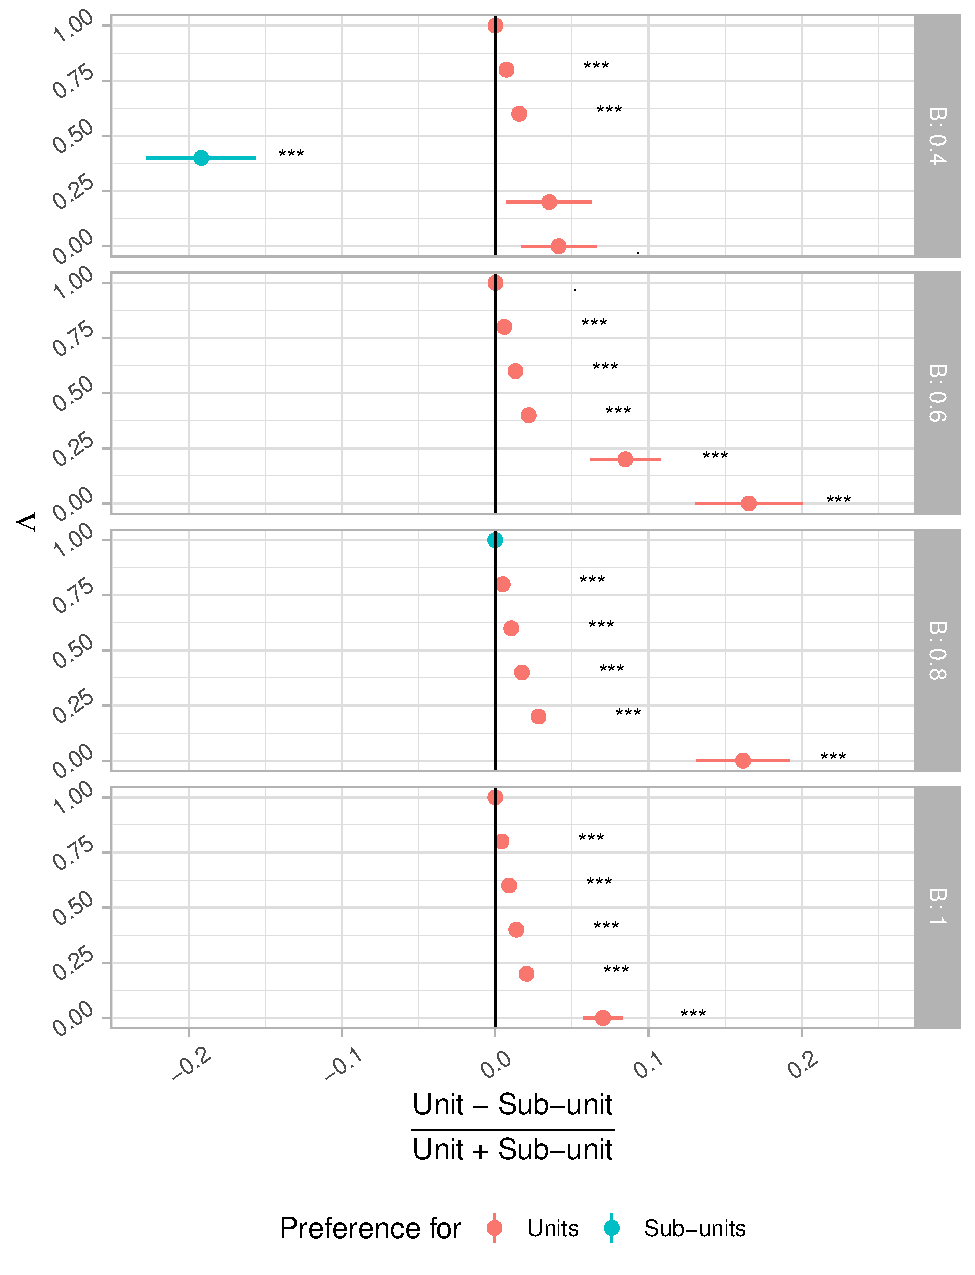
\includegraphics[width=1\linewidth]{tp_model_subunits_files/figure-latex/subunit-experiment-global-create-plot_diff-fw-by-b-average-1} 

}

\caption{Normalized difference scores of network activations after presentation of entire two-syllable units and different types of two-syllable units (i.e., AB and BC from ABC units), as a function of the forgetting rate (y axis) and the interference rate (rows). The rightmost column is the average of the other columns reported by Giroux2009. Positive values indicate stronger activations for units. Significance stars reflect a Wilcoxon test against the chance level of zero. Units generally elicit greater activation compared to AB subunits and compared to the average; when compared to BC units, the sign of the difference score depends on the parameters.}\label{figsubunit-experiment-global-create-plot_diff-fw-by-b-average}
\end{figure}

However, as shown in Figure
\ref{fig:subunit-experiment-global-create-plot_diff-fw-by-b-details},
while units were systematically preferred over \emph{AB} sub-units for
most parameter values, \emph{BC} sub-units could be preferred for very
low or very high interference rates.

\begin{figure}

{\centering 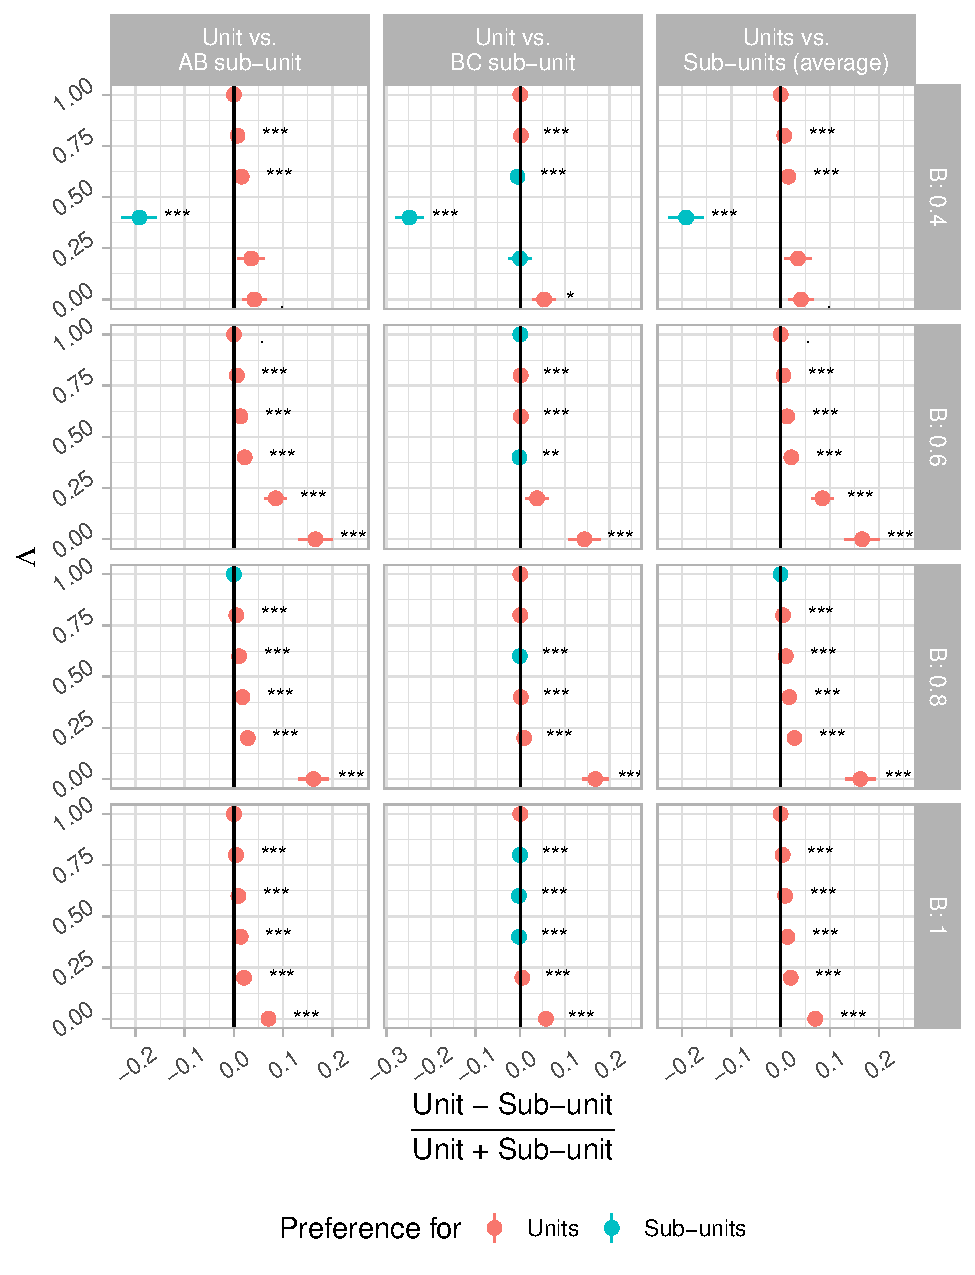
\includegraphics[width=1\linewidth]{tp_model_subunits_files/figure-latex/subunit-experiment-global-create-plot_diff-fw-by-b-details-1} 

}

\caption{Normalized difference scores of network activations after presentation of entire two-syllable units and different types of two-syllable units (i.e., AB and BC from ABC units), as a function of the forgetting rate (y axis) and the interference rate (rows). The rightmost column is the average of the other columns reported by Giroux2009. Positive values indicate stronger activations for units. Significance stars reflect a Wilcoxon test against the chance level of zero. Units generally elicit greater activation compared to AB subunits and compared to the average; when compared to BC units, the sign of the difference score depends on the parameters.}\label{figsubunit-experiment-global-create-plot_diff-fw-by-b-details}
\end{figure}

0 `\emph{\textbf{' 0.001 '}' 0.01 '}' 0.05 `.' 0.1 ' ' 1

To support our contention that the preference for units over sub-units
might arise from the interplay between learning (and thus excitation)
and inhibition, we plot in Figure
\ref{fig:subunit-experiment-global-create-plot_weights} weights between
different pairs of neurons after learning. As suggested above, the
connection between \emph{A} and \emph{C} in a three-syllable \emph{ABC}
unit is generally weaker than other connections, and often substantially
smaller than the interference rate. Depending on the parameter values,
(second order) activation of \emph{C} might thus suppress activation in
\emph{AB} sub-units, and activation of \emph{A} might suppress
activation in \emph{BC} sub-units. However, the exact computational
mechanisms, as well as the differences in behavior betwee \emph{AB} and
\emph{BC} sub-units deserve further investigation. For the current
purposes, we just conclude that the fact that a simple Hebbian learning
model can account for a preference for units over sub-units demonstrates
that such results do not provide evidence that units have been placed in
memory.

\begin{figure}

{\centering 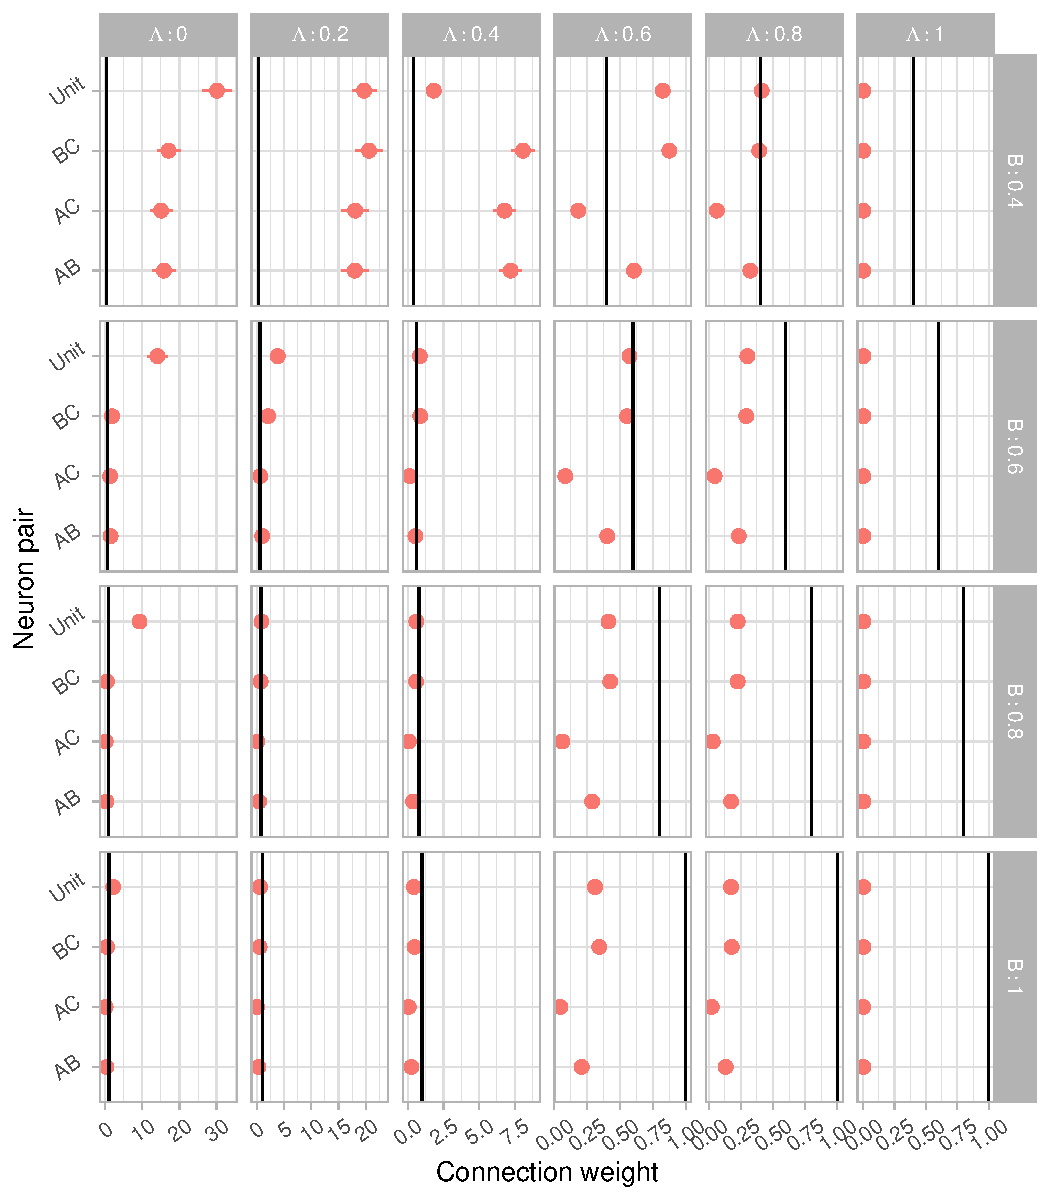
\includegraphics[width=1\linewidth]{tp_model_subunits_files/figure-latex/subunit-experiment-global-create-plot_weights-1} 

}

\caption{Connection weights between different pairs of neurons as a function of the forgetting rate (columns) and the interference rate (rows). The figure shows connection weights within a trisyllabic unit (ABC) and a bisyllabic unit (BC). The black line represents the interference rate. The A-C connection is generally smaller than the other connections, and often substantially smaller than the interference rate.}\label{figsubunit-experiment-global-create-plot_weights}
\end{figure}

  \bibliography{/Users/endress/ansgar.bib}

\end{document}
